\documentclass[a4paper, 10pt]{report}
\usepackage[italian]{babel}
\usepackage[T1]{fontenc}
\usepackage[utf8]{inputenc}
\usepackage{charter}
\usepackage{amsmath}
\usepackage{amsthm}
\usepackage{amsfonts}
\usepackage{graphicx}
\usepackage{wrapfig}
\usepackage{tcolorbox}
\usepackage{fancyhdr}
\usepackage{longtable}

\usepackage{geometry}
\geometry{a4paper, left=2cm,right=2cm,top=2cm,bottom=2cm}

\pagestyle{fancy}
\lhead{}
\chead{}
\rhead{\bfseries 14 ottobre 2019}
\lhead{\bfseries Basi di dati}

\begin{document}

\begin{longtable}{| p{.15\textwidth} | p{.80\textwidth} |}
\textbf{Identificatore di identità} & Un identificatore di entità è unn'insieme di proprietà (attributi/relazioni) che consente di identificare univocamente le istanze di un'identità.

Nell'insieme $I(E)$ non possono esistere due istanze con gli stessi valori (o occorrenze collegate nelle proprietà che fanno parte dell'identificatore). 

L'identificatore si rappresentato con un PALLINO PIENO. 

Gli identificatori si dividono in:
\begin{itemize}
\item[-]Identificatori interni:

\begin{center}
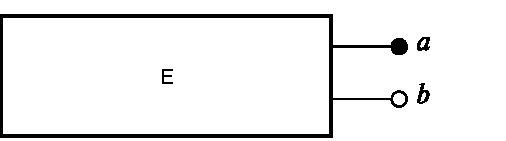
\includegraphics[scale=0.55]{14ottobre02.pdf}
\end{center}

(Non possono esistere due istanze di $E$ con $a$ uguale)

\begin{center}
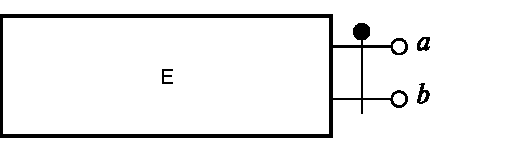
\includegraphics[scale=0.55]{14ottobre03.pdf}
\end{center}

(Non possono esistere due istanze di $E$ con $a_1 == a_2$ e $b_1 == b_2$ uguale)

\begin{center}
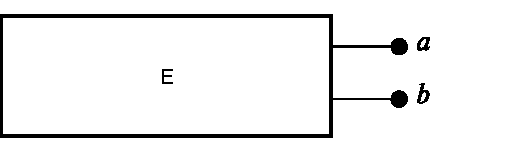
\includegraphics[scale=0.55]{14ottobre04.pdf}
\end{center}

(Non possono esistere due istanze di $E$ con $a_1 == a_2$ o $b_1 == b_2$ uguale)

\item[-] Identificatori esterni:

\begin{center}
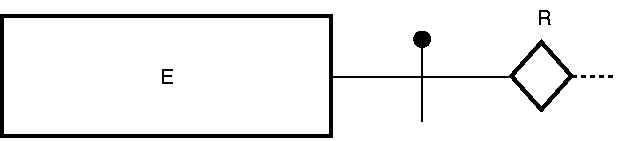
\includegraphics[scale=0.55]{14ottobre05.pdf}
\end{center}

(Non possono esistere due istanze di $E$ con collegate alla relazione $R$)

\begin{center}
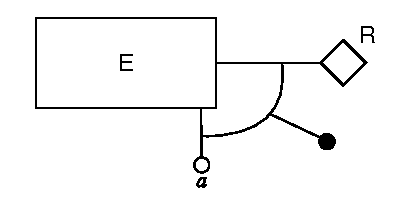
\includegraphics[scale=0.65]{14ottobre06.pdf}
\end{center}

(Non possono esistere due istanze di $E$ con collegate alla relazione $R$ con $a$ uguale oppure entrambe con $a$ uguale collegate a $R$)

\begin{center}
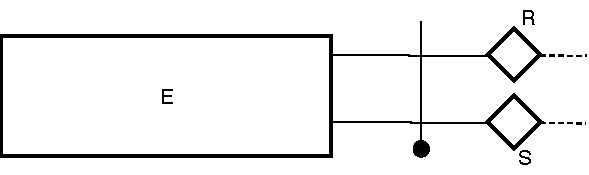
\includegraphics[scale=0.55]{14ottobre07.pdf}
\end{center}

(Non possono esistere due istanze di $E$ collegate sia ad $R$ che ad $S$)

\end{itemize}
\end{longtable}

\newpage

\begin{center}
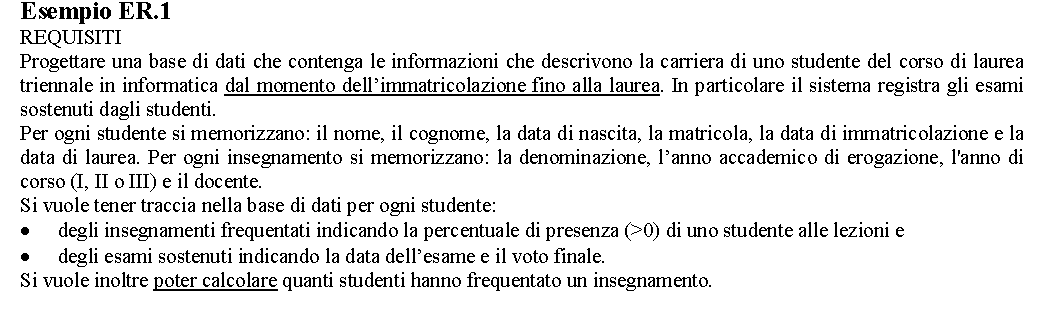
\includegraphics[scale=1]{esercizio.pdf}
\end{center}

\begin{center}
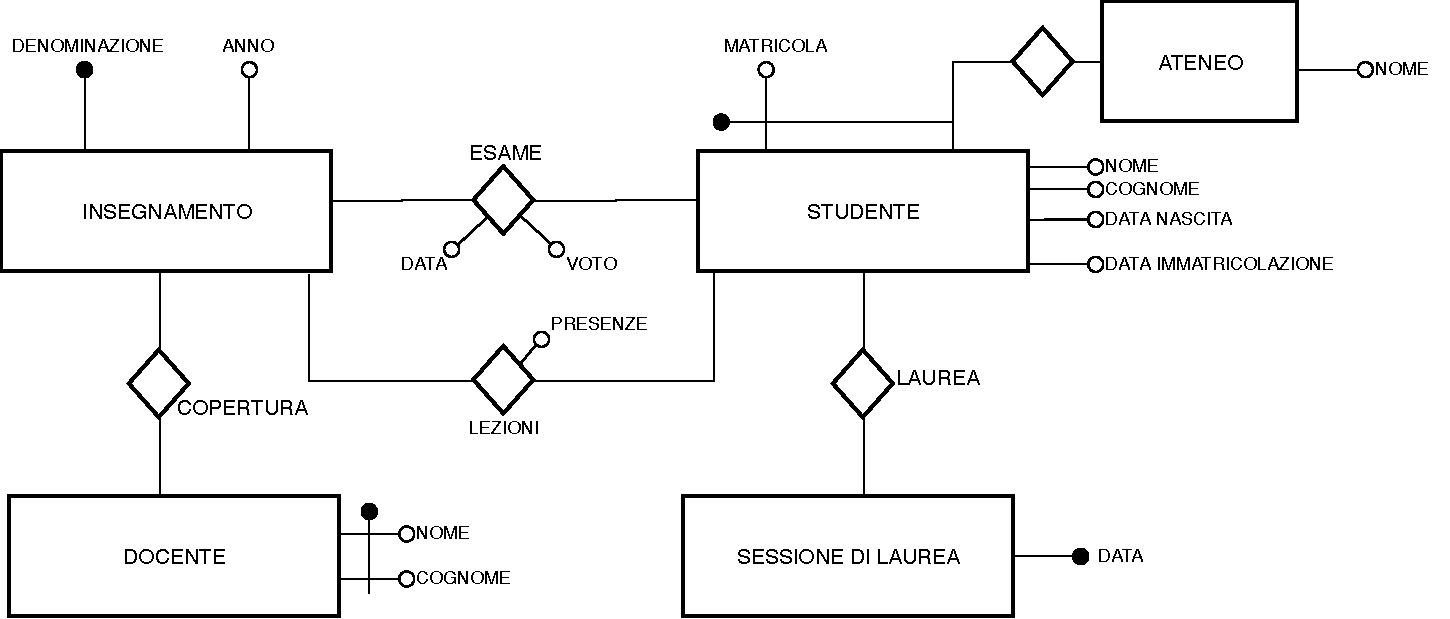
\includegraphics[scale=0.7]{14ottobre01.pdf}
\end{center}

\end{document}